
\section{Additional Evaluation Details}
\label{sec-appendix}
\subsection{Diversity of reasoning models}

Our core analysis focuses on the 20 most representative (non-reasoning) language models.
We additionally evaluate OpenAI and Google reasoning models (o3, o3-mini, and Gemini-2.5-flash) for which inference-time reasoning effort can be set.

\obtodo[id=nb-reasoning-models, created=2025-03-14T08:20:00.000Z, updated=2025-03-23T11:49:02.000Z, completed=2025-03-23T11:49:02.000Z]{Appendix: o3, o3-mini, Gemini-2.5-flash at low vs high reasoning effort.}
\obcomment[kind=result]{Gemini reasoning budget barely moves NoveltyBench. OpenAI: more reasoning effort, less diversity and less utility. Keep this in the appendix, it is not the main 20-model claim.}

\begin{figure}[h]
\centering
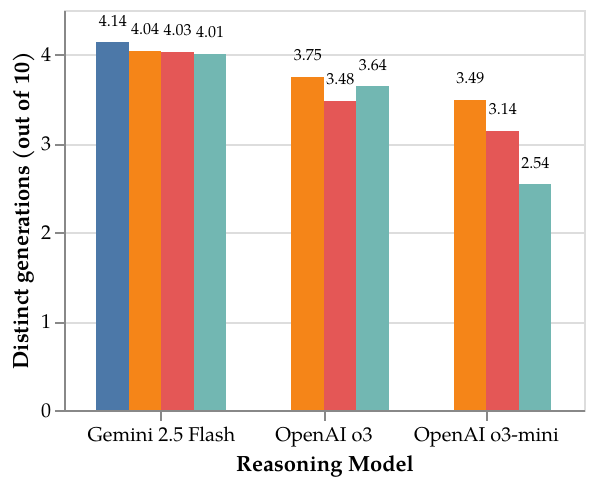
\includegraphics[width=0.49\linewidth]{figures/reasoning_diversity_bars.png}
\hfill
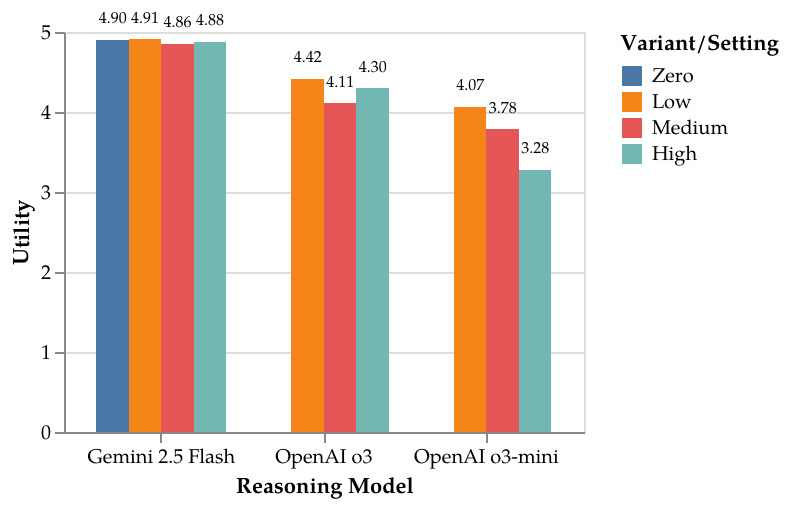
\includegraphics[width=0.49\linewidth]{figures/reasoning_utility_bars.png}
\caption{Diversity and utility of reasoning models on NoveltyBench.
OpenAI's models show reduced diversity and utility as reasoning effort increases.}
\label{fig:reasoning}
\end{figure}

For Gemini, setting the reasoning budget had minimal effect (Figure~\ref{fig:reasoning}).
On OpenAI's models, additional reasoning seems to lead to less diverse and less useful outputs.
Although reasoning models are usually used to solve problems with a single correct answer, preserving diversity is still critical for inference-time scaling strategies such as pass@$k$.

\subsection{Prompt for selecting diverse prompts}

The following system prompt was used with GPT-4o to select prompts from WildChat:

\begin{quote}
\small
You are helping select prompts for a benchmark that measures language models' ability to generate diverse, high-quality alternative answers.
For a prompt to qualify, it should: (1)~allow diverse responses; (2)~be in English, with an English response; (3)~request a natural language response, not code or images; (4)~make a single clearly interpretable request.
Classify the following prompt based on these criteria, and format the provided prompt.
\end{quote}

\subsection{Example prompts from NB-WildChat}

Random samples include: dating-app about-me copy; a collage-composition question; a campus-director narrative inquiry background; ``How can I learn to code?''; ``What are the best free VPNs?''

\subsection{Equivalence classification methods}

On a validation set of 100 pairs, DeBERTa reached the highest AUC (0.81), outperforming fine-tuned GPT-3.5-turbo, GPT-4o-mini, BLEU, ROUGE, and BERTScore.
After choosing an operating threshold, the fine-tuned DeBERTa model has accuracy 71.0\%--79\% depending on the reported checkpoint and F1 $0.811$.

\begin{figure}[h]
\centering
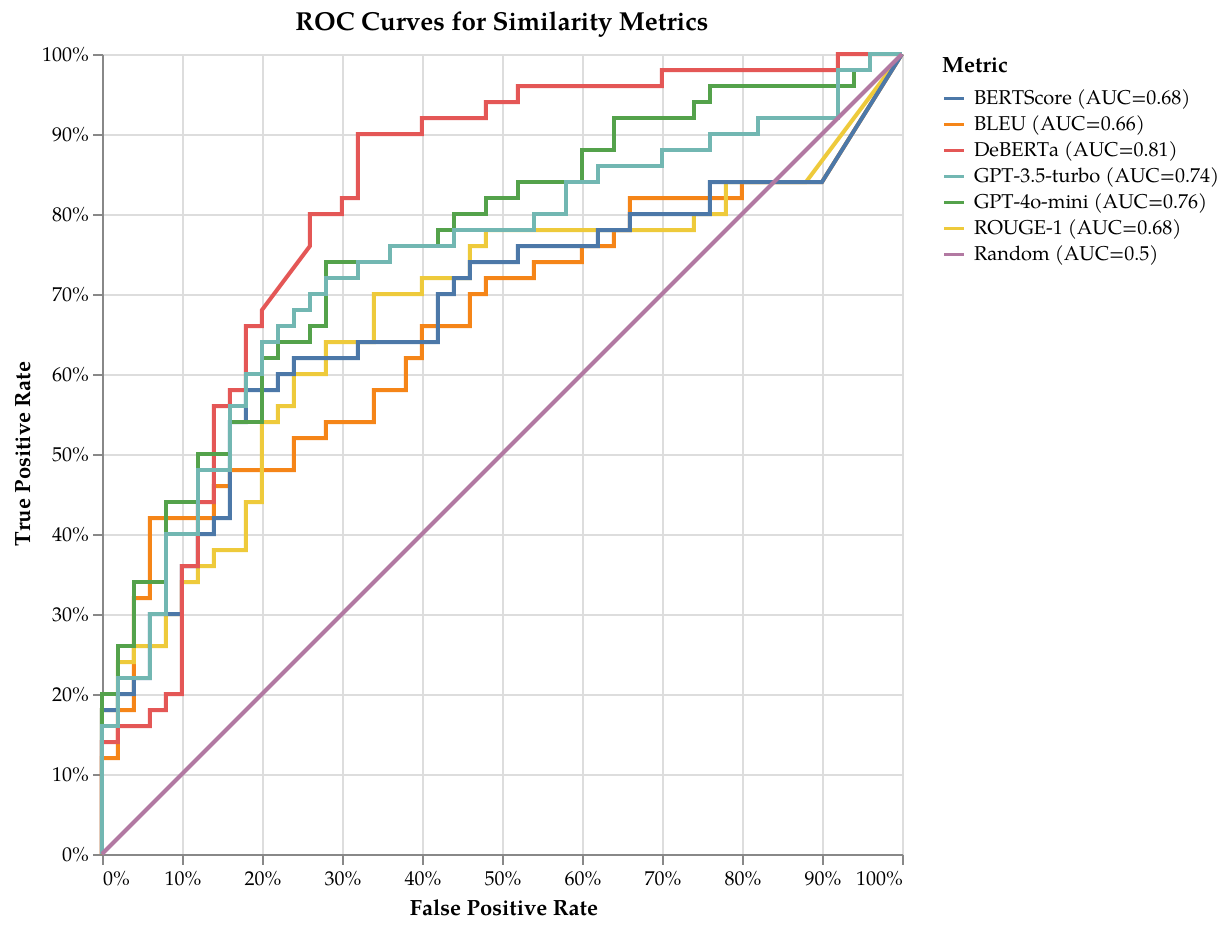
\includegraphics[width=0.8\linewidth]{figures/roc.png}
\caption{ROC curve for various similarity classification methods.}
\label{fig:classifier}
\end{figure}

\subsection{Human annotations}

Eight annotators from our institution responded to each NB-Curated prompt.
The human pool does not collapse to a single mode the way GPT-4o does (Table~\ref{tab:human}).

\begin{table}[h]
\centering
\small
\caption{Human responses to prompts from NB-Curated.}
\label{tab:human}
\begin{tabular}{p{0.22\linewidth}p{0.22\linewidth}p{0.12\linewidth}p{0.28\linewidth}}
\toprule
Filly name & Fields Medal & d20 & Best car 2023 \\
\midrule
Jumpy & Kunihiko Kodaira & 17 & Subaru BRZ \\
Maximus & Akshay Venkatesh & 18 & Honda Civic \\
Oolong & James Maynard & 9 & Toyota Camry \\
Winter & Gerd Faltings & 20 & 2025 Rivian R1S \\
Teazle & Maryam Mirzakhani & 7 & Prius \\
Tony & Maryna Viazovska & 20 & Mazda CX5 \\
Monte & June Huh & 19 & Tesla Model Y \\
Greg & Maryam Mirzakhani & 13 & Volvo XC90 \\
\bottomrule
\end{tabular}
\end{table}
